\documentclass[11pt]{article}

\usepackage[margin=1.2in]{geometry}
\usepackage{booktabs}
\usepackage{graphicx}
\usepackage{hyperref}
\usepackage{amsmath}
\usepackage{array}
\usepackage{float}
\setlength{\parskip}{6pt}
\setlength{\parindent}{0pt}

\hypersetup{colorlinks=true, linkcolor=black, urlcolor=blue, citecolor=black}

\title{Mantis IP Visualization: Patent Dataset Overview\\
\large HUPD and Lens pipelines, datasets, and schemas}
\author{Mantis IP Visualization}
\date{May 2026}

\begin{document}
\maketitle
\tableofcontents
\newpage

% ─────────────────────────────────────────────────────────────────────────────
\section{Introduction}
% ─────────────────────────────────────────────────────────────────────────────

This document covers the two patent datasets we loaded for Mantis: the Harvard USPTO
Patent Dataset (HUPD) and a targeted export from Lens.org. For each one we describe
what the source is, how we pulled and cleaned a usable subset, and what the resulting
files look like. The Lens section also covers how we produced \texttt{US-lens-clean.json}
(US-only records, cleaned and flattened) and \texttt{lens-db-translated.json} (the
broader multilingual export translated to English).

% ═════════════════════════════════════════════════════════════════════════════
\part{Harvard USPTO Patent Dataset (HUPD)}
% ═════════════════════════════════════════════════════════════════════════════

% ─────────────────────────────────────────────────────────────────────────────
\section{What is HUPD?}
% ─────────────────────────────────────────────────────────────────────────────

HUPD is a collection of 4.5 million US patent applications filed between 2004 and 2018,
stored with the original inventor-submitted text rather than the final granted version.
It includes both accepted and rejected applications across all technology domains, which
makes it well-suited for patentability work.

% ─────────────────────────────────────────────────────────────────────────────
\section{What's in the full dataset}
% ─────────────────────────────────────────────────────────────────────────────

Each record is a JSON file with 26 fields:

\begin{center}
\small
\begin{tabular}{ll}
  \toprule
  \textbf{Field} & \textbf{What it is} \\
  \midrule
  \texttt{application\_number}   & USPTO application identifier \\
  \texttt{publication\_number}   & Publication number once the app is published \\
  \texttt{title}                 & Short title of the invention \\
  \texttt{decision}              & \texttt{ACCEPTED}, \texttt{REJECTED}, or \texttt{PENDING} \\
  \texttt{date\_produced}        & Date the record was produced internally \\
  \texttt{date\_published}       & Date the application was published \\
  \texttt{filing\_date}          & Date filed with the USPTO \\
  \texttt{patent\_issue\_date}   & Date granted (if accepted) \\
  \texttt{abandon\_date}         & Date abandoned (if applicable) \\
  \texttt{patent\_number}        & Granted patent number (if accepted) \\
  \texttt{main\_cpc\_label}      & Primary CPC code \\
  \texttt{cpc\_labels}           & All CPC codes \\
  \texttt{main\_ipcr\_label}     & Primary IPC code \\
  \texttt{ipcr\_labels}          & All IPC codes \\
  \texttt{uspc\_class}           & US Patent Classification class \\
  \texttt{uspc\_subclass}        & US Patent Classification subclass \\
  \texttt{examiner\_id}          & USPTO examiner ID \\
  \texttt{examiner\_name\_last}  & Examiner last name \\
  \texttt{examiner\_name\_first} & Examiner first name \\
  \texttt{examiner\_name\_middle}& Examiner middle name \\
  \texttt{inventor\_list}        & Inventors (name, city, state, country) \\
  \texttt{abstract}              & Abstract as written by the applicant \\
  \texttt{claims}                & Claims section \\
  \texttt{background}            & Background of the invention \\
  \texttt{summary}               & Summary of the invention \\
  \texttt{full\_description}     & Full description as filed \\
  \bottomrule
\end{tabular}
\end{center}

The data is split into per-year \texttt{.tar.gz} archives, roughly 62\,GB uncompressed in total.

% ─────────────────────────────────────────────────────────────────────────────
\section{How we got our 2k sample}
% ─────────────────────────────────────────────────────────────────────────────

\subsection{Sampling approach}

The Hugging Face \texttt{datasets} loader no longer works with recent library versions,
so we pulled records directly from the per-year archives over HTTP via \texttt{data-load.py},
reading them as streams to avoid downloading the full 62\,GB. We took roughly 140 records
from the front of each year's archive (2004--2018), shuffled, and trimmed to 2,100.
Archive order within a year is unsorted by application number, so this is a reasonable
stand-in for a random draw.

\subsection{Data cleaning}

Records with fewer than 25 words in the abstract were dropped---anything shorter is a
stub or formatting artifact. The 2,100 records here were already pre-filtered, so all
2,100 remain.

\subsection{Final dataset at a glance}

\begin{table}[H]
  \centering
  \begin{tabular}{ll}
    \toprule
    \textbf{Property} & \textbf{Value} \\
    \midrule
    Total records           & 2,100 \\
    Filing years covered    & 2004--2018 (15 years) \\
    Records per year        & $\sim$140 (roughly even) \\
    Fields per record       & 26 \\
    Unique examiners        & 1,777 \\
    Mean inventors/patent   & 2.74 \\
    Mean IPC labels/patent  & 2.08 \\
    Abstract: median length & 110 words \\
    Claims: median length   & 821 words \\
    Full description: median & 5,998 words \\
    Total words (full desc.) & $\sim$17.8 million \\
    \bottomrule
  \end{tabular}
  \caption{Summary statistics for the HUPD 2k sample.}
  \label{tab:hupd_summary}
\end{table}

\texttt{title}, \texttt{abstract}, \texttt{claims}, and \texttt{full\_description} are
all present in 100\% of records. \texttt{background} is present in 94.6\% and
\texttt{summary} in 93.3\%---both can be legitimately absent on older or shorter applications.

% ─────────────────────────────────────────────────────────────────────────────
\section{The data in detail}
% ─────────────────────────────────────────────────────────────────────────────

\subsection{IPC and CPC classification codes}

\textbf{IPC (International Patent Classification)} is the older WIPO system, present on
93.7\% of records. Codes are hierarchical: a letter for the top-level section, a
two-digit class, a subclass letter, and further subdivisions. \texttt{G06F}, for example,
is G~(Physics) $\to$ 06~(Computing) $\to$ F~(Electrical digital data processing).

\textbf{CPC (Cooperative Patent Classification)} was introduced jointly by the USPTO and
EPO around 2013, so it only covers 40.2\% of the sample---roughly the filings from 2013
onward. It follows the same letter-section structure as IPC.

The eight top-level WIPO sections:

\begin{center}
\small
\begin{tabular}{cl}
  \toprule
  \textbf{Section} & \textbf{What it covers} \\
  \midrule
  A & Human Necessities \\
  B & Operations and Transport \\
  C & Chemistry and Metallurgy \\
  D & Textiles and Paper \\
  E & Fixed Constructions \\
  F & Mechanical Engineering \\
  G & Physics / Computing \\
  H & Electricity / Electronics \\
  \bottomrule
\end{tabular}
\end{center}

The top 20 IPC subclasses by primary label count:

\begin{center}
\small
\begin{tabular}{llr}
  \toprule
  \textbf{Subclass} & \textbf{Description} & \textbf{Count} \\
  \midrule
  G06F & Electrical digital data processing & 176 \\
  H01L & Semiconductor devices & 117 \\
  A61K & Medical / dental / personal care preparations & 76 \\
  H04L & Transmission of digital information & 70 \\
  H04N & Pictorial communication & 61 \\
  A61B & Diagnosis / surgery / medical instruments & 51 \\
  H04W & Wireless communications networks & 42 \\
  G01N & Investigating materials & 39 \\
  G06Q & Data processing for administrative / commercial purposes & 37 \\
  A61F & Implants / prosthetics & 28 \\
  G02B & Optical elements & 27 \\
  G06K & Graphical data reading / recognition & 27 \\
  H04B & Transmission (general) & 24 \\
  B41J & Selective printing mechanisms & 23 \\
  A61M & Devices for introducing media into the body & 19 \\
  G11C & Static stores (memory) & 19 \\
  H05K & Printed circuits / manufacture of assemblies & 19 \\
  G03G & Electrography / electrophotography & 18 \\
  H01R & Electrically-conductive connections & 17 \\
  F16H & Gearing & 16 \\
  \bottomrule
\end{tabular}
\end{center}

\subsection{Category and outcome distributions}

The sample skews toward G~(Physics) and H~(Electricity), consistent with the general
trend in US filings over this period. All eight sections are represented. Computing
(G06F) is the largest subclass, followed by semiconductors (H01L) and pharmaceuticals
(A61K). There are 319 distinct subclasses in total.

\begin{figure}[H]
  \centering
  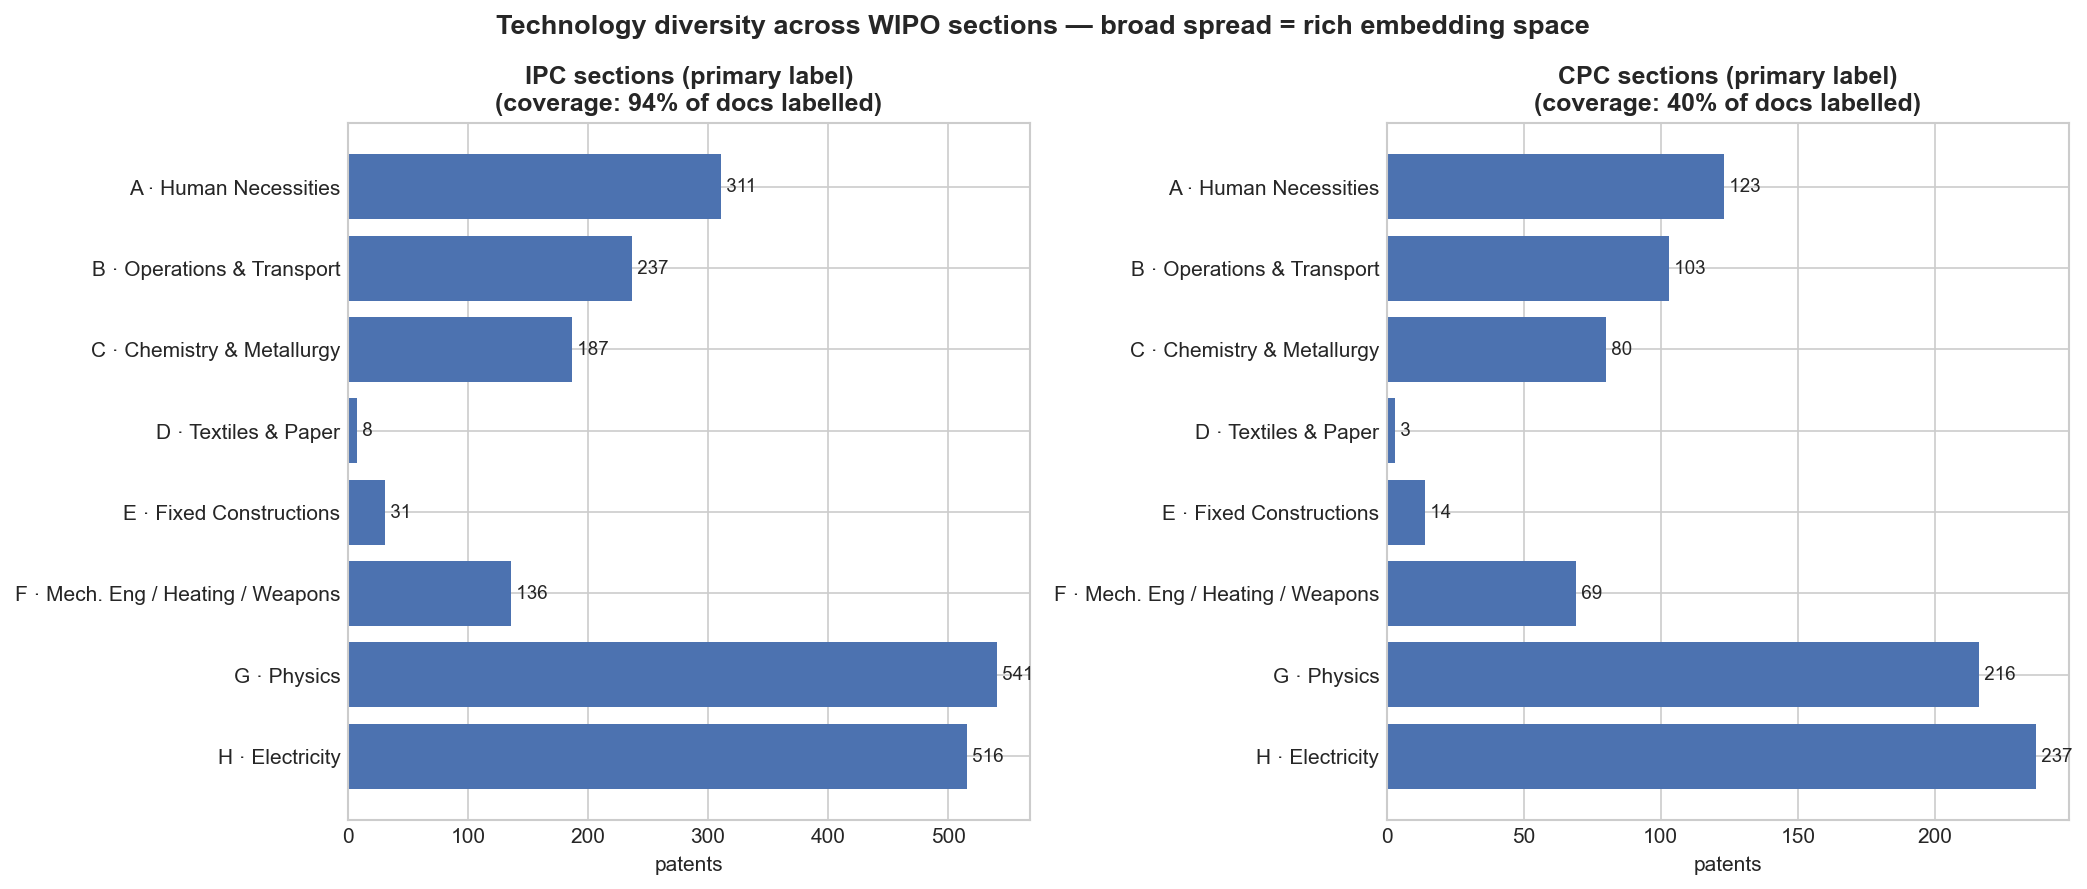
\includegraphics[width=0.95\textwidth]{harvard-uspto/summary/figures/fig01_ipc_cpc_sections.png}
  \caption{Distribution across the eight WIPO top-level sections for IPC (94\% coverage)
  and CPC (40\% coverage).}
  \label{fig:hupd_ipc_cpc}
\end{figure}

\begin{figure}[H]
  \centering
  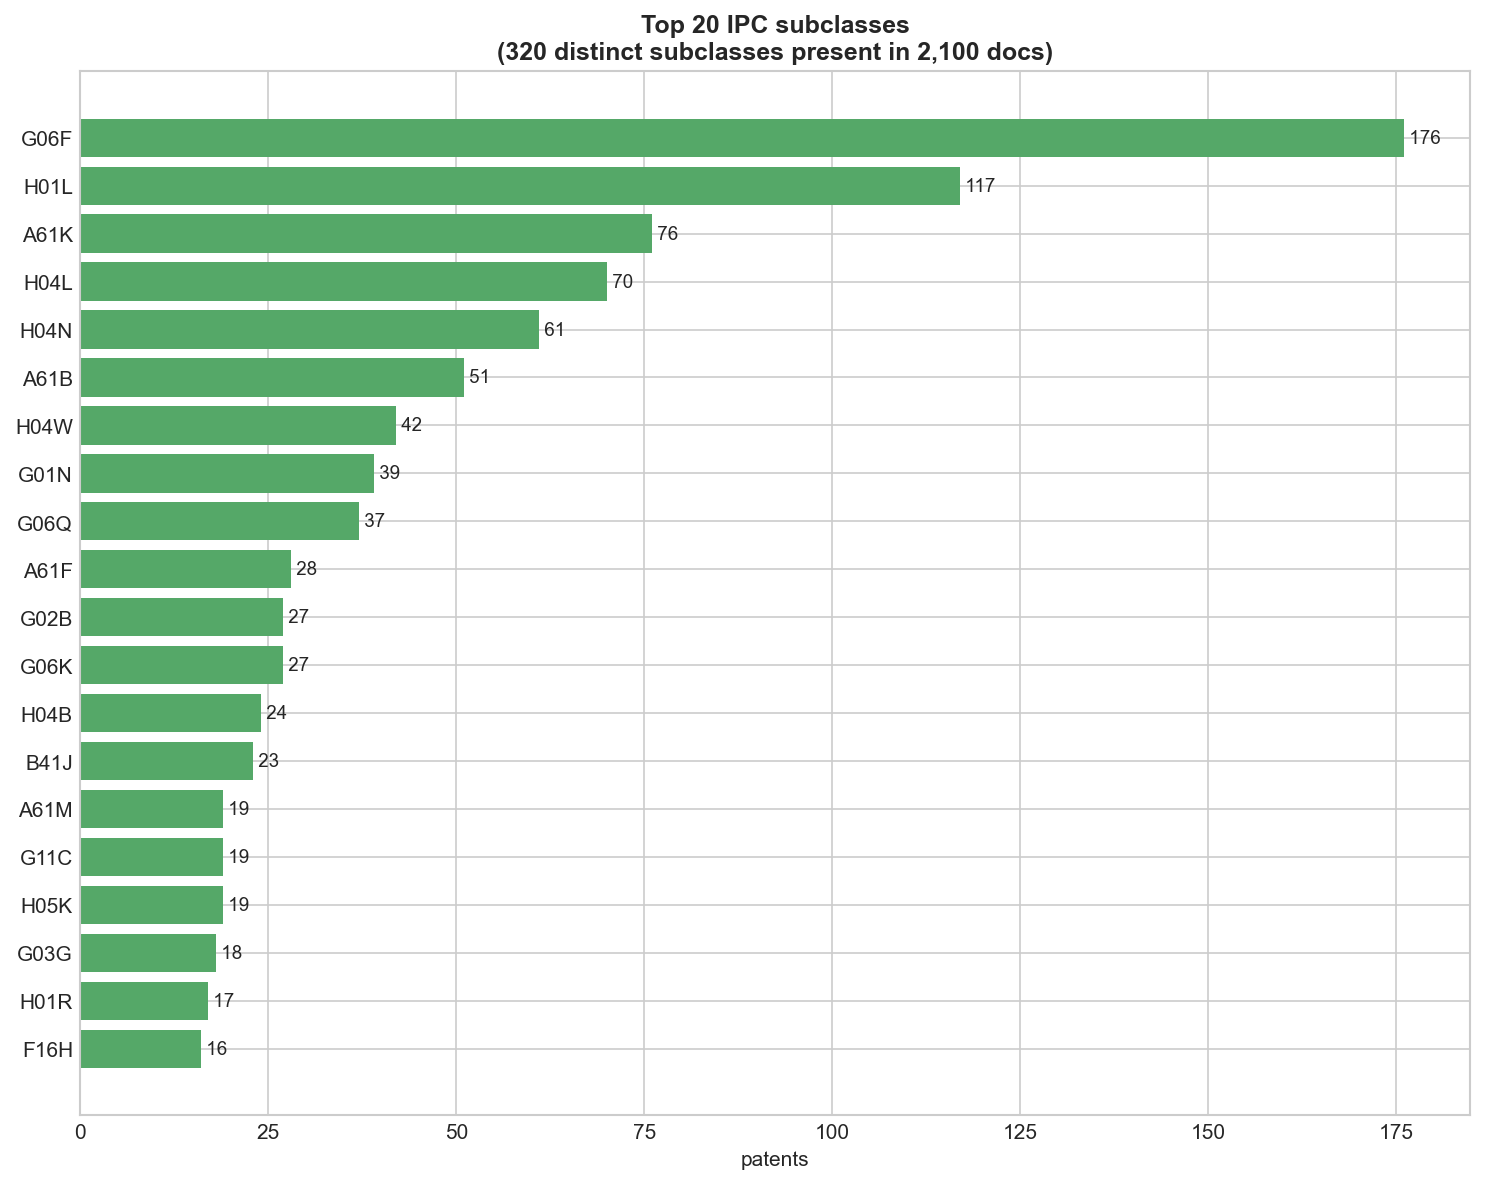
\includegraphics[width=0.95\textwidth]{harvard-uspto/summary/figures/fig02_top_ipc_subclasses.png}
  \caption{Top 20 IPC subclasses (319 distinct subclasses present overall).}
  \label{fig:hupd_ipc_subclasses}
\end{figure}

Just over half the sample (54.6\%) was accepted, about a quarter (25.9\%) rejected, and
19.6\% are still pending. The pending share rises sharply from 2016 onward---those
applications had not resolved when the dataset was frozen in 2022.

\begin{figure}[H]
  \centering
  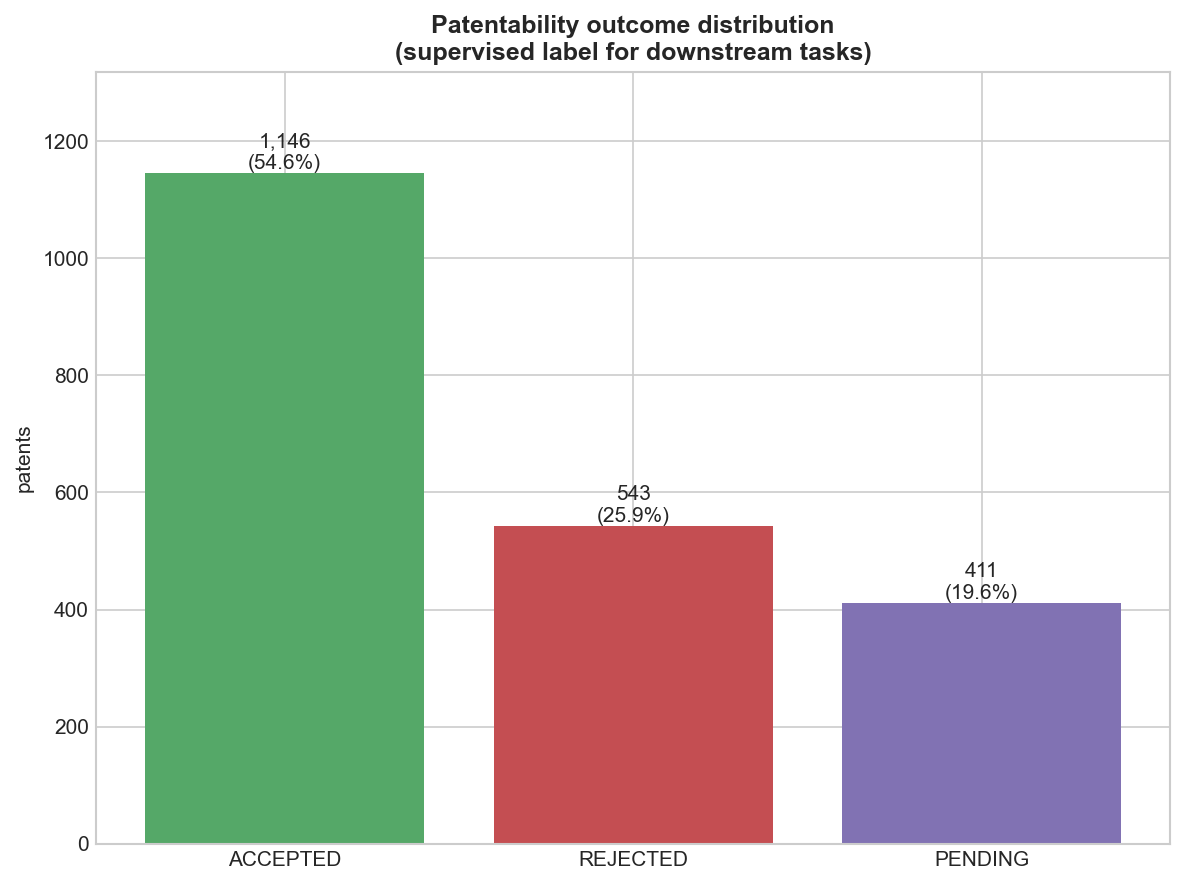
\includegraphics[width=0.72\textwidth]{harvard-uspto/summary/figures/fig03_decision_distribution.png}
  \caption{Patentability outcomes across the 2,100-record sample.}
  \label{fig:hupd_decisions}
\end{figure}

\begin{figure}[H]
  \centering
  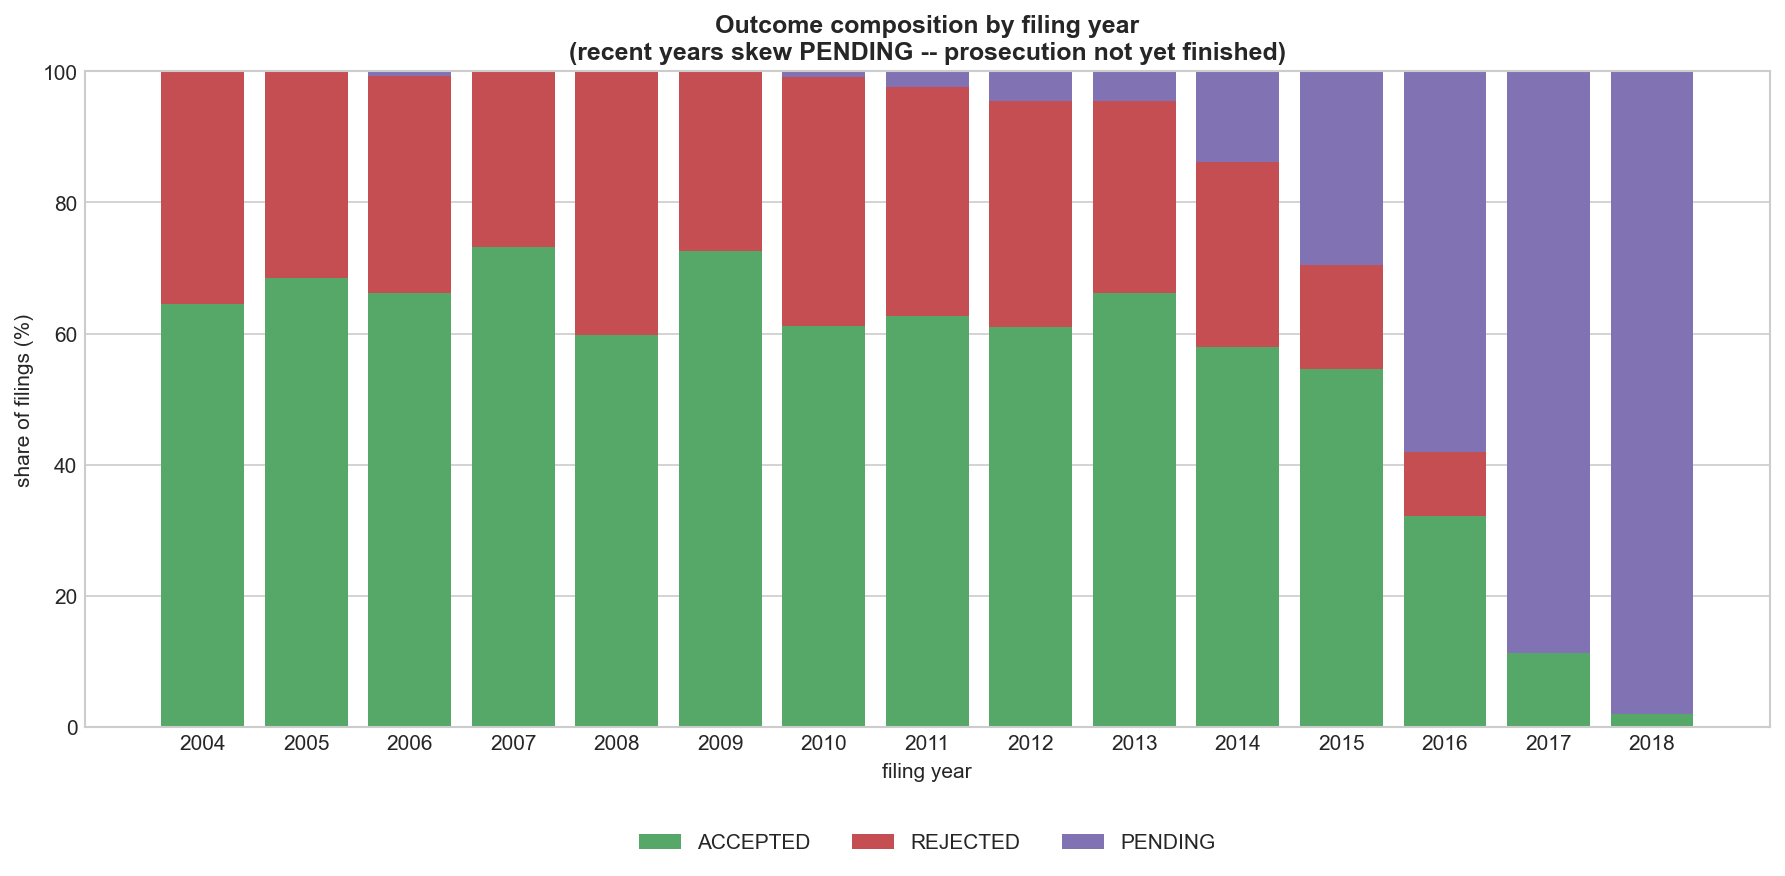
\includegraphics[width=0.95\textwidth]{harvard-uspto/summary/figures/fig04_decision_by_year.png}
  \caption{Outcome composition by filing year. Recent years skew PENDING because
  prosecution had not finished when the dataset was frozen.}
  \label{fig:hupd_decision_by_year}
\end{figure}

\subsection{Text length details}

\begin{table}[H]
  \centering
  \begin{tabular}{lrrrrrr}
    \toprule
    \textbf{Field} & \textbf{Non-empty} & \textbf{Mean} & \textbf{Median} &
    \textbf{Std} & \textbf{p90} & \textbf{Max} \\
    \midrule
    title            & 100\% &  8    &    7  &    5  &     14  &     44 \\
    abstract         & 100\% & 111   &  110  &   43  &    151  &    405 \\
    claims           & 100\% & 964   &  821  &  723  &  1,655  & 11,589 \\
    background       &  95\% & 483   &  345  &  584  &  1,040  &  9,290 \\
    summary          &  93\% & 742   &  415  & 1,277 &  1,624  & 22,730 \\
    full\_description & 100\% & 8,466 & 5,998 & 8,871 & 15,435 & 131,338 \\
    \bottomrule
  \end{tabular}
  \caption{Word-count statistics per text field. There are notable outliers throughout.}
  \label{tab:hupd_text_lengths}
\end{table}

% ═════════════════════════════════════════════════════════════════════════════
\part{Lens Patent Database}
% ═════════════════════════════════════════════════════════════════════════════

% ─────────────────────────────────────────────────────────────────────────────
\section{What is the Lens Dataset?}
% ─────────────────────────────────────────────────────────────────────────────

Lens.org is a free, open-access patent search platform run by Cambia. It pulls records
from the USPTO, EPO, WIPO, JPO, CNIPA, and more---over 150 million patents total. Each
record has bibliographic metadata, legal status, family linkages, classification codes,
and (where available) abstract, description, and claims. The Lens API supports bulk JSON
export, which is how we got our data.

% ─────────────────────────────────────────────────────────────────────────────
\section{What's in the raw dataset}
% ─────────────────────────────────────────────────────────────────────────────

The raw export (\texttt{lens-raw.jsonl}) has \textbf{8,357 records} from a targeted
query on IP relevant to Mantis. Records span 43 jurisdictions and 20 languages, running
from the late 19th century through 2024, though the bulk are from 2020 onward.

\subsection{Jurisdictions and languages}

Non-US records make up the majority of the pull, with China, Japan, and the EPO being
the largest non-US sources (see Figure~\ref{fig:lens_jurisdiction}). The multilingual
character is a direct result of the broad query scope and gets resolved during cleaning.

\begin{figure}[H]
  \centering
  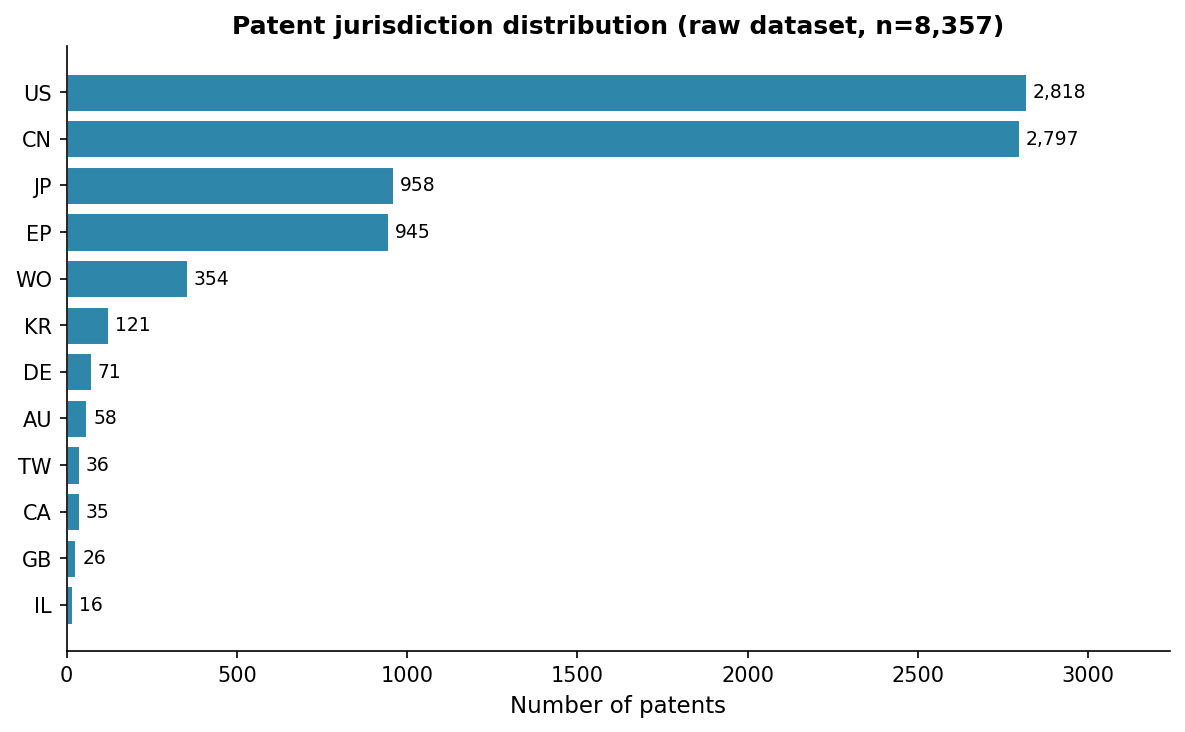
\includegraphics[width=0.92\textwidth]{lens-db/summary/figures/fig1_jurisdiction.png}
  \caption{Jurisdiction distribution (top 12 offices, n\,=\,8,357).}
  \label{fig:lens_jurisdiction}
\end{figure}

\begin{figure}[H]
  \centering
  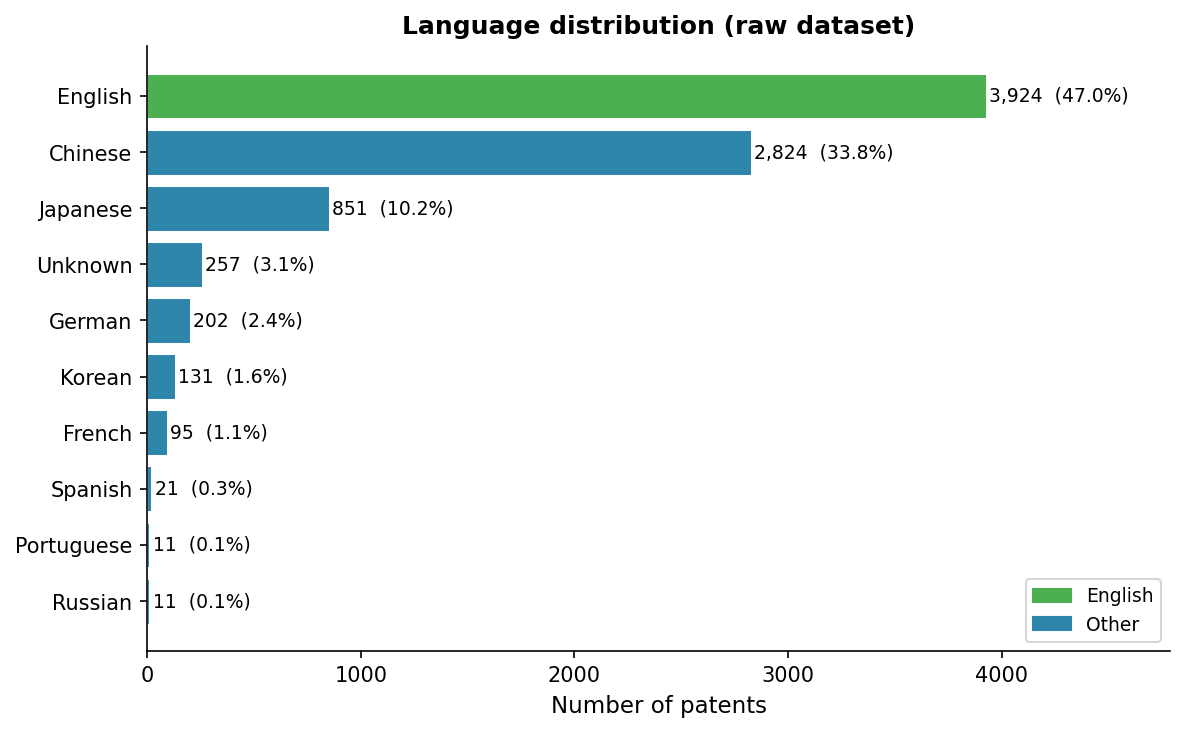
\includegraphics[width=0.92\textwidth]{lens-db/summary/figures/fig2_language.png}
  \caption{Language distribution across the raw dataset.}
  \label{fig:lens_language}
\end{figure}

\subsection{Field completeness}

The abstract is the most reliably present field. Description and claims are missing from
over half of records---normal for non-US or older filings. The sequence listing field has
almost no coverage and was dropped.

\begin{figure}[H]
  \centering
  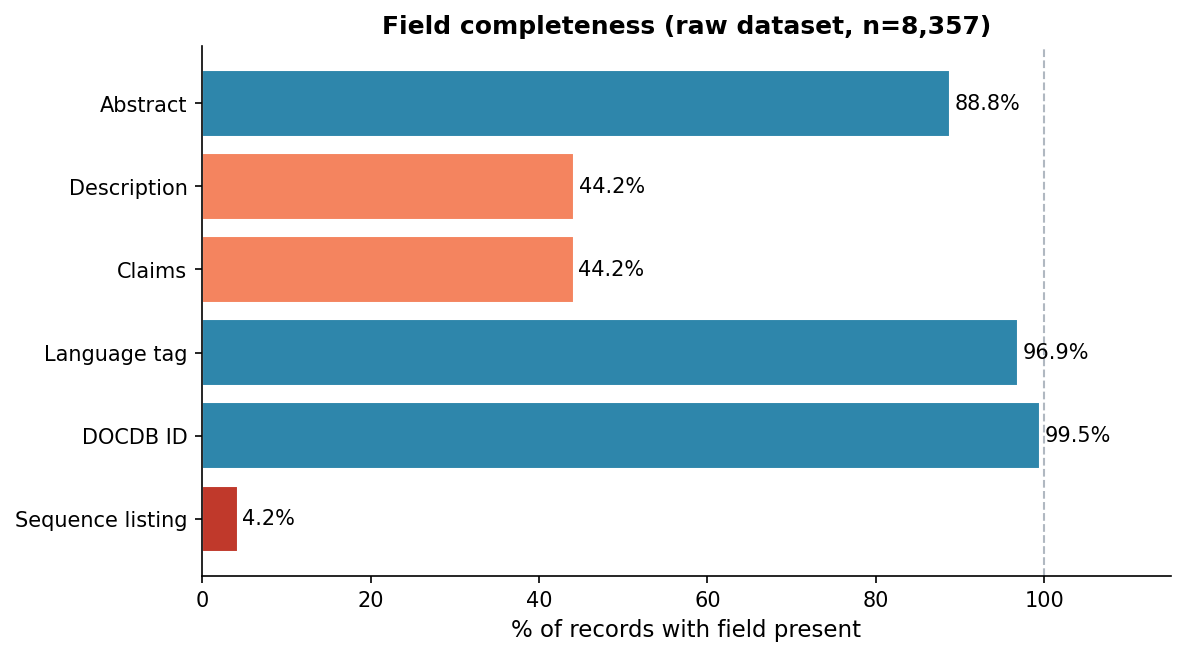
\includegraphics[width=0.92\textwidth]{lens-db/summary/figures/fig4_field_completeness.png}
  \caption{Percentage of raw records with each field populated.}
  \label{fig:lens_completeness}
\end{figure}

\subsection{Publication types and legal status}

The dataset mixes applications and granted patents. Most are either active or pending,
reflecting the recency of the pull.

\begin{figure}[H]
  \centering
  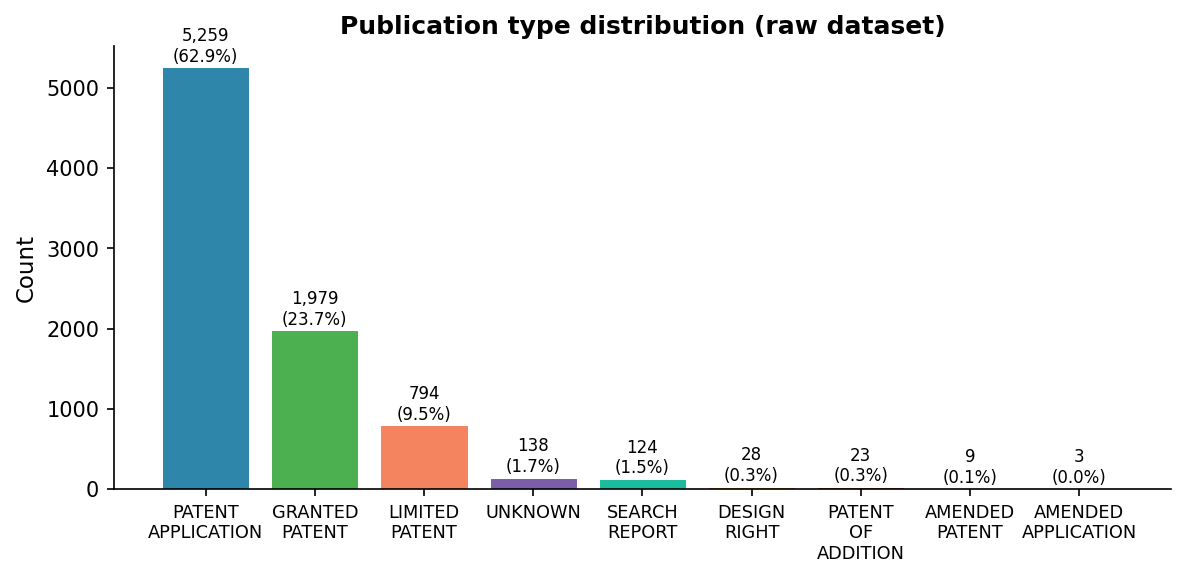
\includegraphics[width=0.92\textwidth]{lens-db/summary/figures/fig5_publication_type.png}
  \caption{Publication type distribution.}
  \label{fig:lens_pubtype}
\end{figure}

\begin{figure}[H]
  \centering
  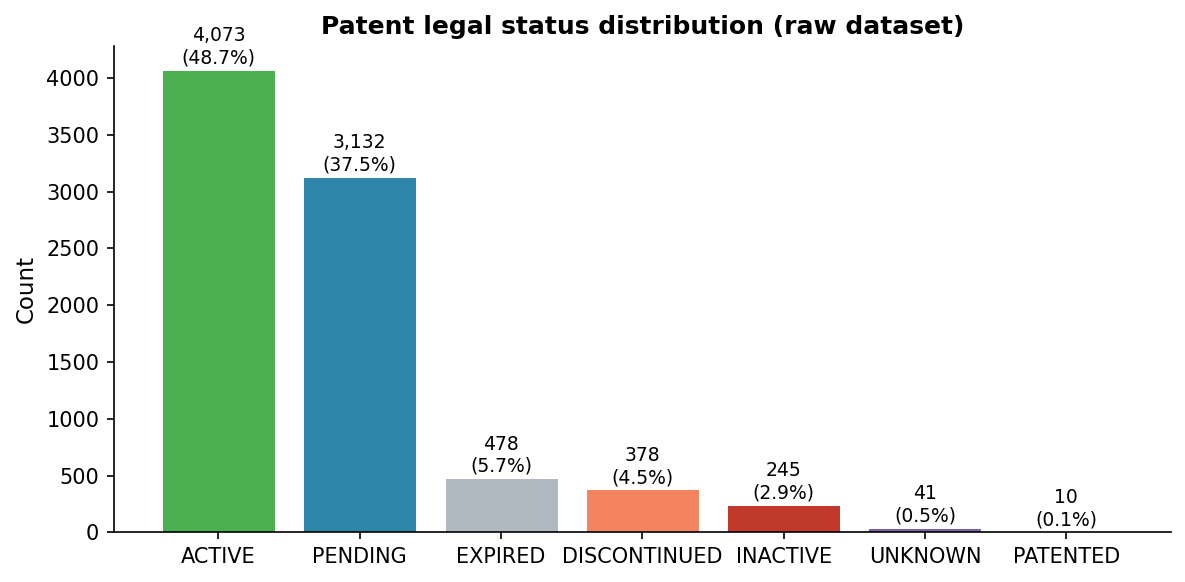
\includegraphics[width=0.92\textwidth]{lens-db/summary/figures/fig6_patent_status.png}
  \caption{Legal status distribution.}
  \label{fig:lens_status}
\end{figure}

\subsection{Publication year}

The dataset is heavily weighted toward recent filings, with most records from 2020 onward
and a thin historical tail going back to the 19th century.

\begin{figure}[H]
  \centering
  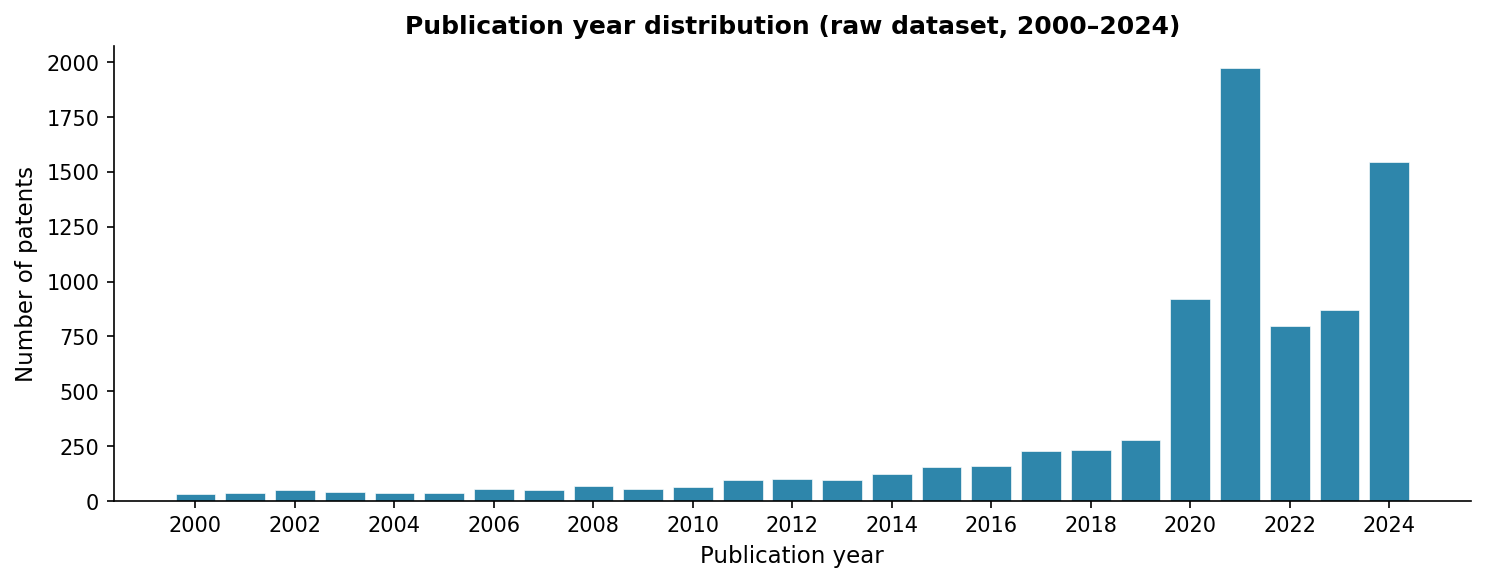
\includegraphics[width=0.92\textwidth]{lens-db/summary/figures/fig7_publication_year.png}
  \caption{Publication year distribution (2000--2024).}
  \label{fig:lens_year}
\end{figure}

\subsection{Technology coverage (IPC sections)}

All eight WIPO sections are present. G~(Physics / Computing) and H~(Electricity) have
the highest counts, consistent with the Mantis technology focus.

\begin{figure}[H]
  \centering
  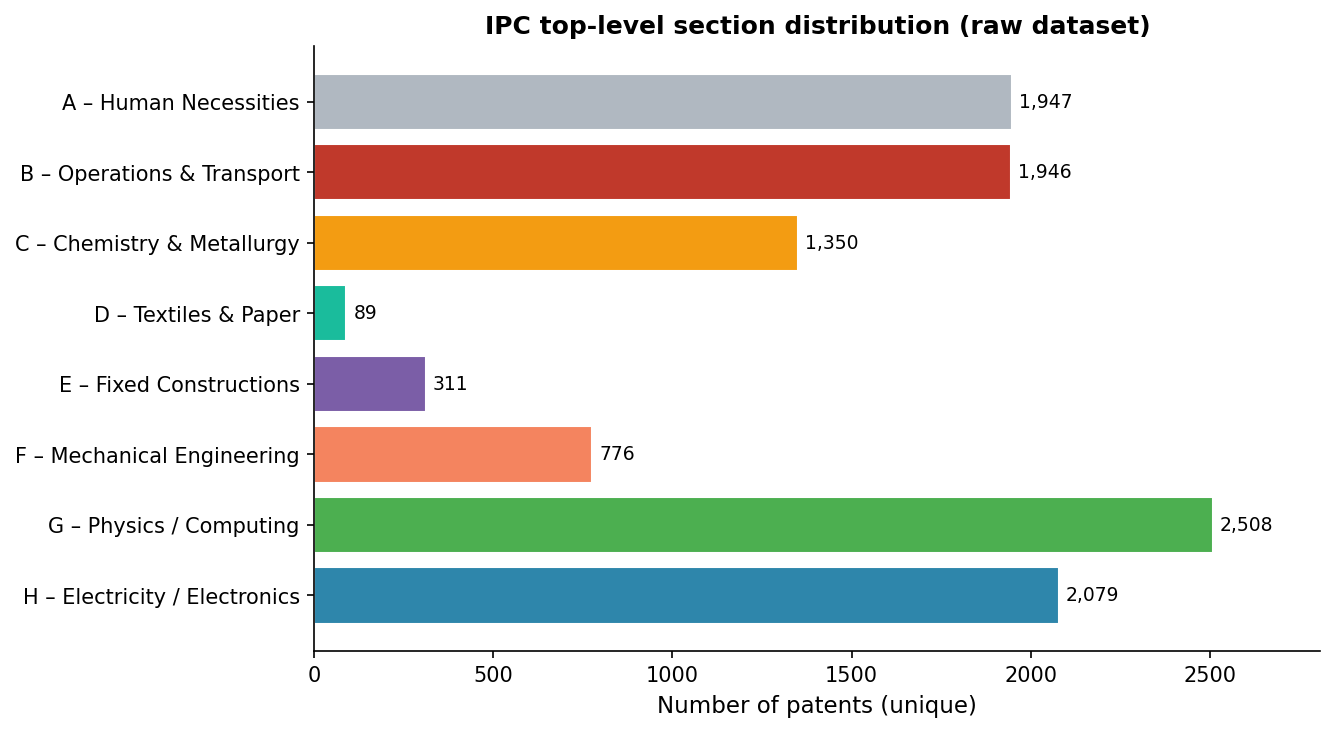
\includegraphics[width=0.92\textwidth]{lens-db/summary/figures/fig8_ipc_sections.png}
  \caption{Unique patents per IPC top-level section (a patent may appear in multiple).}
  \label{fig:lens_ipc}
\end{figure}

% ─────────────────────────────────────────────────────────────────────────────
\section{Producing \texttt{US-lens-clean.json}}
\label{sec:lens_cleaning}
% ─────────────────────────────────────────────────────────────────────────────

Starting from \texttt{lens-raw.jsonl}, we applied three sequential filters and then
flattened the nested JSON schema to produce \texttt{US-lens-clean.json}.

\subsection{Filtering}

\begin{enumerate}
  \item \textbf{US jurisdiction only.} Dropping non-US records cut the dataset from 8,357
    to 2,818 and, as a side effect, resolved the language issue: 99.9\% of what remained
    was in English (three records had no language tag but are presumed English given their
    US jurisdiction).

  \item \textbf{Abstract required.} The abstract is Mantis's primary semantic signal, so
    records without one were dropped. Only 39 of the 2,818 US records lacked an abstract,
    leaving 2,779.

  \item \textbf{Deduplication.} Records were deduplicated on \texttt{lens\_id}. No
    duplicates were found, so the count stayed at 2,779.
\end{enumerate}

\begin{center}
\begin{tabular}{lr}
  \toprule
  \textbf{Stage} & \textbf{Records} \\
  \midrule
  Raw \texttt{lens-raw.jsonl} & 8,357 \\
  US jurisdiction only & 2,818 \\
  Abstract present & 2,779 \\
  Deduplicated & 2,779 \\
  \bottomrule
\end{tabular}
\end{center}

\subsection{Schema flattening}

Lens records are deeply nested---inventor names, for instance, are buried at
\texttt{biblio > parties > inventors > extracted\_name > value}. \texttt{clean.py}
flattens everything to a single-level schema of 19 fields, dropping any fields that are
redundant or not relevant for patent identification or semantic analysis. Missing values
are filled with the string \texttt{"Null"} so every record has the same shape.

% ─────────────────────────────────────────────────────────────────────────────
\section{Final dataset at a glance}
\label{sec:lens_final}
% ─────────────────────────────────────────────────────────────────────────────

\begin{table}[H]
  \centering
  \begin{tabular}{ll}
    \toprule
    \textbf{Property} & \textbf{Value} \\
    \midrule
    Total records             & 2,779 \\
    Jurisdiction              & US only \\
    Language                  & English (99.9\%), unknown (0.1\%) \\
    Fields per record         & 19 \\
    Records with abstract     & 2,779 (100\%) \\
    Records with description  & 1,196 (43.0\%) \\
    Abstract: mean length     & 105 words \\
    Abstract: median length   & 107 words \\
    Abstract: 90th pctile     & 149 words \\
    \bottomrule
  \end{tabular}
  \caption{Summary statistics for \texttt{US-lens-clean.json}.}
  \label{tab:lens_summary}
\end{table}

% ─────────────────────────────────────────────────────────────────────────────
\section{Schema reference}
\label{sec:lens_schema}
% ─────────────────────────────────────────────────────────────────────────────

\begin{table}[H]
  \centering
  \small
  \begin{tabular}{p{4.8cm} p{7.5cm}}
    \toprule
    \textbf{Field} & \textbf{Description} \\
    \midrule
    \texttt{lens\_id}                    & Globally unique Lens.org record identifier. \\
    \texttt{jurisdiction}                & Patent office (always \texttt{US} here). \\
    \texttt{doc\_number}                 & USPTO document number. \\
    \texttt{kind}                        & Publication stage code (e.g., \texttt{A}, \texttt{B2}). \\
    \texttt{date\_published}             & Publication date (YYYY-MM-DD). \\
    \texttt{lang}                        & Language of the document. \\
    \texttt{publication\_type}           & e.g., \texttt{PATENT\_APPLICATION}, \texttt{GRANTED\_PATENT}. \\
    \texttt{patent\_status}              & e.g., \texttt{ACTIVE}, \texttt{PENDING}, \texttt{EXPIRED}. \\
    \texttt{title}                       & Invention title(s); may include multiple translations. \\
    \texttt{application\_date}           & Date filed with the USPTO. \\
    \texttt{priority\_date}              & Earliest priority claim date. \\
    \texttt{applicants}                  & Applicant / assignee names. \\
    \texttt{inventors}                   & Inventor names. \\
    \texttt{ipc\_classifications}        & IPC classification symbols. \\
    \texttt{cited\_by\_lens\_ids}        & Forward citations (Lens IDs). \\
    \texttt{simple\_family\_lens\_ids}   & Simple patent family members (Lens IDs). \\
    \texttt{extended\_family\_lens\_ids} & Extended patent family members (Lens IDs). \\
    \texttt{abstract}                    & Full abstract text. \\
    \texttt{description}                 & Full description text, where available. \\
    \bottomrule
  \end{tabular}
  \caption{The 19 fields in \texttt{US-lens-clean.json}. Missing values are stored as \texttt{"Null"}.}
  \label{tab:lens_schema}
\end{table}

% ─────────────────────────────────────────────────────────────────────────────
\section{Producing \texttt{lens-db-translated.json}}
\label{sec:translation}
% ─────────────────────────────────────────────────────────────────────────────

\texttt{US-lens-clean.json} only keeps US records, which are almost entirely English.
The broader cleaned export still has records in Chinese, Japanese, German, Korean, and
others. To make that dataset usable by English-language models, we produced
\texttt{lens-db-translated.json} by running a translation pass over \texttt{lens-db-clean.json}.

Translation used \textbf{Argos Translate}, a free offline neural machine translation
library. Because translating thousands of records takes significant time, the job was left
running on a VM overnight. For \texttt{title} and \texttt{abstract}---which are stored as
lists of per-language entries in the raw Lens format---the pipeline picks any existing
English entry first and only calls the translator when none is present. The
\texttt{description} field is translated only for records whose language tag is not
already English. After the pass, all text fields are plain strings and every record's
\texttt{lang} is set to \texttt{"en"}.

\end{document}
